%%%%%%%%%%%%%%%%%%%%%%%%%%%%%%%%%%%%%%%%%
% Simple Sectioned Essay Template
% LaTeX Template
%
% This template has been downloaded from:
% http://www.latextemplates.com
%
% Note:
% The \lipsum[#] commands throughout this template generate dummy text
% to fill the template out. These commands should all be removed when 
% writing essay content.
%
%%%%%%%%%%%%%%%%%%%%%%%%%%%%%%%%%%%%%%%%%

%----------------------------------------------------------------------------------------
%	PACKAGES AND OTHER DOCUMENT CONFIGURATIONS
%----------------------------------------------------------------------------------------

\documentclass[11pt]{article} % Default font size is 12pt, it can be changed here

\usepackage{geometry} % Required to change the page size to A4
\geometry{a4paper} % Set the page size to be A4 as opposed to the default US Letter

\usepackage{graphicx} % Required for including pictures
\usepackage{soul,color}

\usepackage{float} % Allows putting an [H] in \begin{figure} to specify the exact location of the figure

\usepackage{hyperref}

\linespread{1} % Line spacing

%\setlength\parindent{0pt} % Uncomment to remove all indentation from paragraphs

\title{\textsc{\LARGE CMSC 676 Information Retrieval} \\ Project - Phase 1 }
\author{Primal Pappachan \\ primal1@umbc.edu}
\date{{\large \today}}

\begin{document}

\maketitle

%----------------------------------------------------------------------------------------
%	INTRODUCTION
%----------------------------------------------------------------------------------------

\section{Introduction} % Major section

In this assignment I have implemented and evaluated the performance of a program to tokenize the documents. Additionally I have compared the performance of my approach with that of another approach (by Jacob Rettiga) in terms of quality of tokens and running time. I have used Python to code the program. To execute the program from a linux terminal 

\begin{verbatim}
$python tokenizer.py files/ out_files/ <n>
\end{verbatim}

The parameters to the code are as follows. The detailed explanation of input parameters can be seen in the next section.

\begin{enumerate}
\item tokenizer.py - Name of the program
\item files - Input directory
\item out\_files - Output Directory
\item n - Number of input files
\end{enumerate}

For example, the following code will execute the tokenizer on 100 files from 'files' directory and write the tokenized output to out\_files directory. 

\begin{verbatim}
$python tokenizer.py files/ out_files/  100
\end{verbatim}

You need to install the NLTK to run the program. Please refer to the documentation\footnote{\url{http://www.nltk.org/install.html}} on how to install NLTK.

%------------------------------------------------

\subsection{Input} % Sub-section

A directory of input documents is given to the program as input from the command line. The documents were html files with primarily ascii content and with some unicode as well. The files were named using three digit numbers starting from 001. For the purpose of evaluation, I added an additional parameter to specify the number of files which should be considered from the total number of files (503).

%------------------------------------------------

\subsection{Output} % Sub-section

The output from program is written to the directory 'out\_files'. This directory contains two subdirectories named 'token\_files' and 'sorted\_files'. The first one contains all the tokenized documents with one output file per input file. Each of these files are named as 'input\_file\_name'.txt, for example the output token file for 001.html is 001.txt. The content of these files are follows, \textit{token {space} frequency}. The second directory contains two files with the complete vocabulary sorted by token and frequency. 

\section{Methodology} % Major section

As earlier mentioned, I used Python to program the tokenizer. I made use of python libraries such as Natural Language Tool Kit (NLTK), re, unicodedata to clean up the text and to build the vocabulary. The steps involved in the process has been outlined in the diagram below.

\begin{figure}[h] % Inline image example
  \begin{center}
    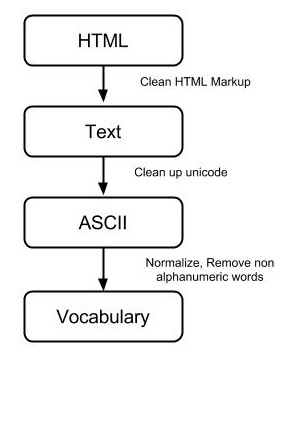
\includegraphics[width=0.38\textwidth]{method.jpg}
  \end{center}
  \caption{Tokenizing Pipeline}
\end{figure}

The main function read the input file directory and traverses it using the os.walk() function which returns the contents of the directory as well as path to the directory. I appended the path to the file names and stored these in a list. Additionally I randomized the order of files in this list by using random.shuffle(). \\

For cleaning up HTML I used the helper function provided by NLTK, nltk.clean\_html(). After passing the HTML string read from the file  to this helper function it returns the raw text. I also built a simple dictionary of special characters which were commonly seen in the documents (\&nbsp, \&quot etc). I used this dictionary to replace the occurrences of special characters with their ASCII equivalents. To convert unicode characters to their ascii equivalents, I used the unicodedata\footnote{\url{http://docs.python.org/2/library/unicodedata.html}} module in python. The normalize function provided by this module returns the normal form of the unicode string. It takes a parameter form which can be used to specify the value for normal form. I used the form KD (NFKD) which will apply compatibility decomposition i.e replace all compatibility characters with their equivalents. \\

The wordpunct\_tokenize function by NLTK breaks up the cleaned string from earlier step into a list of words. Before building the vocabulary, I lower cased all of the text from the NTLK Text Object by using  by iterating through the list and using String.lower() on each of tokens. Additionally a final check was done using regular expressions to remove any words with non alphanumeric characters. After this step we have the list of words. \\   

To count the occurrences of each word in the list I used the Counter function from collections library in Python. It takes a list as input and returns a dictionary (Python object) with tokens as keys and their frequency as values. This dictionary was unsorted. This was written to a file to complete the tokenization for a single input file. \\

For constructing the complete vocabulary, I used a global dictionary and updated it after each step of individual tokenization i.e for each file. This dictionary was sorted based on keys (tokens) and values (frequencies) and was written to separate files. The following diagram shows the control flow with respect to various modules in the program. The 'word\_sort' and 'freq\_sort' sorts the complete vocabulary by tokens and frequencies respectively after tokenization has been completed for all files. The 'write\_token\_file' function writes tokens from a single input file to a corresponding output file. 

\begin{figure}[h]
  \begin{center}
    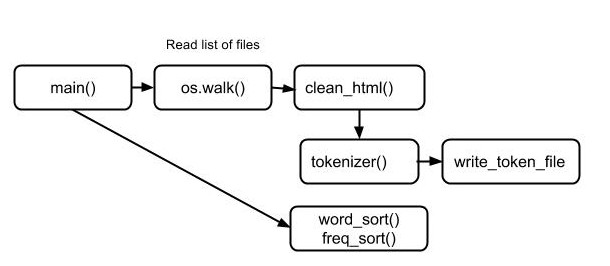
\includegraphics[width=0.5\textwidth]{module.jpg}
  \end{center}
  \caption{Tokenizing Pipeline}
\end{figure}

%------------------------------------------------

\section{Evaluation} % Sub-sub-section

The following graph shows the running time of the program (Tokenizer A). The configuration of the system from the command \textit{lscpu} has been added for reference in the Appendix. For experimentation purpose, I ran the tokenizer 10 times for different number of input files (100, 200, 300, 400, 500) and averaged the results. This was done to smoothen out the effect of different file sizes on the program execution time. As you can see from the graph both the system time and elapsed time increases almost linearly. After profiling the python script using cProfile \footnote{\url{http://docs.python.org/2/library/profile.html}} I saw that the sorted function was most computationally intensive in terms of ratio of total time and number of calls (0.321/4) to the function. But since Python makes use of mergesort for sorting, with increasing number of tokens time taken by it would grow only by nlogn.   

\begin{figure}[h] % Inline image example
  \begin{center}
    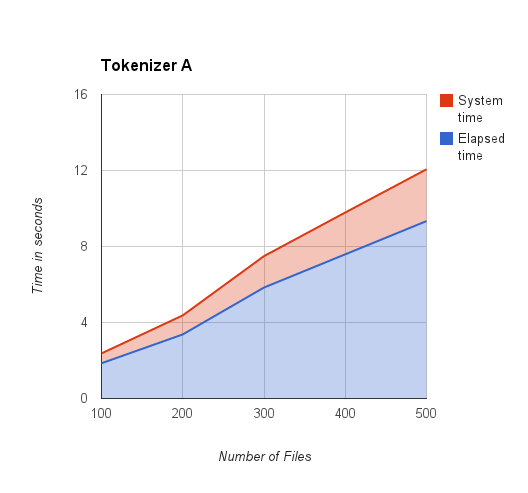
\includegraphics[width=0.6\textwidth]{tokenizerA.png}
  \end{center}
  \caption{Time vs Number of Files}
\end{figure}

%------------------------------------------------

\section{Comparison} % Sub-sub-section

I compared the results with the program of Jacob Rettiga (Tokenizer B) with whom I collaborated in this assignment. The efficiency of his program has been shown below in the graph.   

\begin{figure}[h] % Inline image example
  \begin{center}
    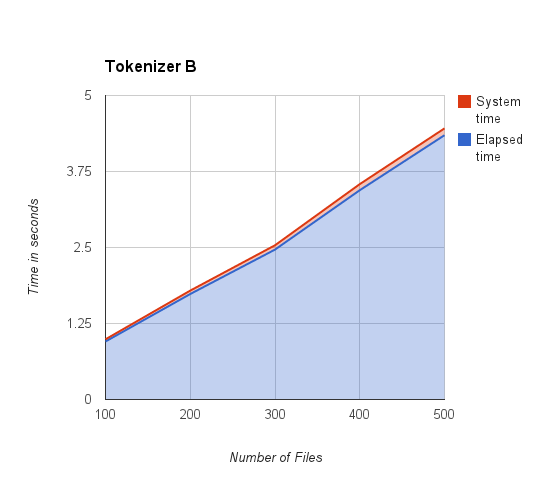
\includegraphics[width=0.6\textwidth]{tokenizerB.png}
  \end{center}
  \caption{Time vs Number of Files}
\end{figure}


\section{Conclusion}

After comparing the results between Tokenizer A and Tokenizer B, we can see that the time taken by both the tokenizers grow linearly with respect to the number of files. Tokenizer A takes more time than Tokenizer B for the same number of files. One of these might be a probable cause for this difference.

\begin{itemize}
\item usage of NLTK in Tokenizer A versus the usage of HTMLParser in Tokenizer B. As HTMLParser is a library lighter than NLTK, it consumes less memory and executes faster
\item Also after comparing the code of both tokenizers, we saw that using a simple counter using a variable is much more efficient than using the Counter Module from Collections library
\end{itemize}

I decided to use NLTK as I had previous experience of using it in my projects and is easy to use. Additionally it provides a suite of tokenizing functions for handling various types of text. The output of both tokenizers were similar in quality as both of us had taken care to clean the meta data as well as converting unicode characters.

The total number of tokens in the complete vocabulary was 128204. 

 \hl{write about number of tokens and comparison between 50 first and last tokens, also change it to new graph, generate new 50 first and last tokens, update README} \\ 



%----------------------------------------------------------------------------------------
%	MAJOR SECTION X - TEMPLATE - UNCOMMENT AND FILL IN
%----------------------------------------------------------------------------------------

%\section{Content Section}

%\subsection{Subsection 1} % Sub-section

% Content

%------------------------------------------------

%\subsection{Subsection 2} % Sub-section

% Content

%----------------------------------------------------------------------------------------
%	CONCLUSION
%----------------------------------------------------------------------------------------

%----------------------------------------------------------------------------------------
%	BIBLIOGRAPHY
%----------------------------------------------------------------------------------------

\begin{thebibliography}{99} % Bibliography - this is intentionally simple in this template

\bibitem http://nltk.googlecode.com/svn/trunk/doc/book/ch03.html
\bibitem http://stackoverflow.com/questions/2600191/how-can-i-count-the-occurrences-of-a-list-item-in-python
\bibitem http://stackoverflow.com/questions/273192/check-if-a-directory-exists-and-create-it-if-necessary
\bibitem http://stackoverflow.com/questions/2365411/python-convert-unicode-to-ascii-without-errors
\bibitem http://www.saltycrane.com/blog/2007/03/python-oswalk-example/
 
\end{thebibliography}

\section{Appendix}

\subsection{System Configuration}

\begin{verbatim}
Architecture:          x86_64
CPU op-mode(s):        32-bit, 64-bit
Byte Order:            Little Endian
CPU(s):                4
On-line CPU(s) list:   0-3
Thread(s) per core:    1
Core(s) per socket:    4
Socket(s):             1
NUMA node(s):          1
Vendor ID:             GenuineIntel
CPU family:            6
Model:                 58
Stepping:              9
CPU MHz:               1600.000
BogoMIPS:              6385.15
Virtualization:        VT-x
L1d cache:             32K
L1i cache:             32K
L2 cache:              256K
L3 cache:              6144K
NUMA node0 CPU(s):     0-3
\end{verbatim}

%----------------------------------------------------------------------------------------

\end{document}